\documentclass[a4paper,12pt]{article} %style de document
\usepackage[utf8]{inputenc} %encodage des caractères
\usepackage[french]{babel} %paquet de langue français
\usepackage[T1]{fontenc} %encodage de la police
\usepackage{times}
\usepackage[top=2cm,bottom=2cm,left=2cm,right=2cm]{geometry} %marges
\usepackage{graphicx} %'affichage des images
\usepackage{enumitem}
\usepackage{hyperref}
\usepackage{fancyhdr}
\pagestyle{fancy}
\usepackage{amssymb}
\usepackage[useregional]{datetime2}
\usepackage{datetime}
\usepackage{listings}
\newdateformat{monthyeardate}


\usepackage[linesnumbered,french,ruled,onelanguage]{algorithm2e}%linesnumbered permet de numeroter les lignes, ruled permet un affichage avec des lignes separatrices
\lstset{
    keywords=[2]{/*}
    keywordstyle=[2]\color{pink}
}

\fancyhead[L]{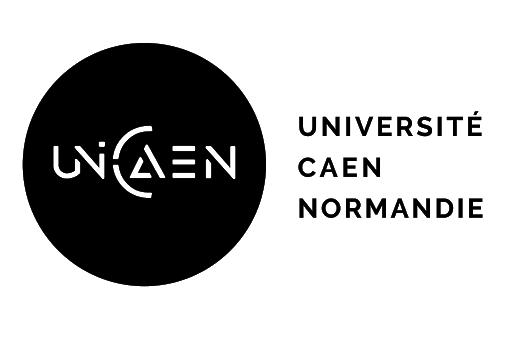
\includegraphics[scale = 0.15]{unicaen.png}}
\fancyhead[C]{}
\fancyhead[R]{Lancer de Rayon\vspace*{0.5em}}

\renewcommand{\headrulewidth}{0pt}
\renewcommand{\footrulewidth}{1pt}

\fancyfoot[R]{\textbf{page \thepage}}
\fancyfoot[C]{}
\fancyfoot[L]{Dans le cadre de l'évaluation Licence 2 Informatique}

\usepackage{verbatim}

\author{Guillaume LEMONNIER\\Erin LE DREAU\\Harisson KOBYLT\\Antoine LEMAITRE\\Logan VIVEN\\\\L2 info, 2021-2022\\Groupe 4A}
\title{Lancer de Rayon}

\begin{document}

\maketitle

\newpage

\vspace*{0.5em}

\tableofcontents

\newpage

\section{Introduction}

Le lancer de rayon est une technique de visualisation 3D reoposant sur le principe de calculer la distance de l'écran avec un objet afin de connaitre sa taille et donc ça représentation sur l'écran.
Cette technique de visualisation 3D est très utilisé dans le domaine de l'informatique, elle est connue sous le nom de Ray Tracing.

\subsection{Objectif}

Lors de notre selection de projet nous avons vite pensé à choisir ce projet. En effet il s'agissait du projet qui nous inspiré le plus parmis tout ceux proposé.
Nous nous sommes répartit le travail comme suit :

\vspace*{1em}

\centerline {
    \begin{tabular}{|c|c|}
    \hline
        Guillaume LEMONNIER & Model 3D et Rayons\\
        \hline
        Antoine LEMAITRE & Lumières et Ombres\\
        \hline
        Harisson KOBYLT & Interface\\
        \hline
        Logan VIVEN & Parser\\
        \hline
        Erin LE DREAU & Interface\\
    \hline
    \end{tabular}
}

\vspace*{1em}

De ce fait nous nous somme répartit le travail équitablement. Cependant comme il est possible de le voir.
Erin et Harisson se sont retrouvé sur la même partie. La raison est que Erin n'avait à l'origine pas de groupe.
Elle nous a rejoint au bout du cours numéro 3 et nous avons donc du la mettre avec quelqu'un, car le travail été déjà équitablement répartit.

L'objectif était donc de programmer le principe du schema suivant :

\vspace*{1em}

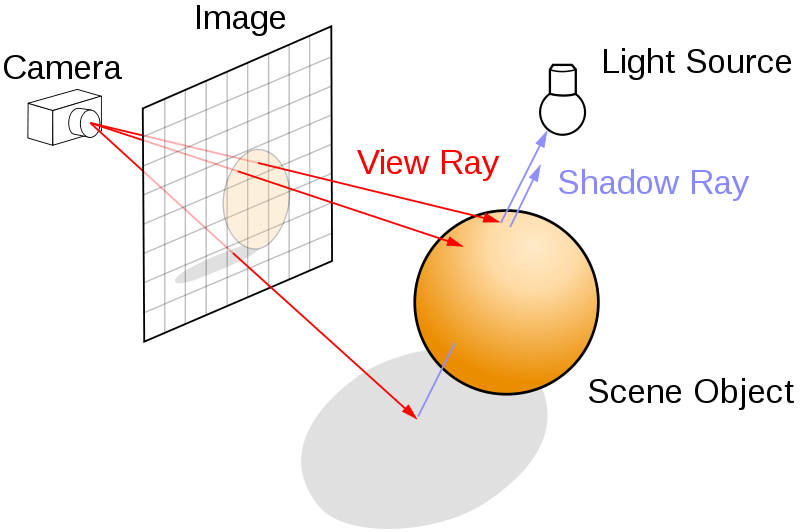
\includegraphics[scale = 0.5]{raytracing.png}

\newpage

\section{Partie Guillaume}

\subsection{ray}

Lors de la première séance nous avons mis sur le papier nos rôles.
Guillaume, ayant déjà une bonne idée de ce qu'il devait faire, a commencé les Vector2D, Vector3D et Ray qu'il a fini pendant la première séance sans trop de difficultées.

\subsubsection{Vector2D}

\begin{algorithm}
    \caption{constructor}\label{Vector2D:constructor1}
    $this.(0, 0)$\;
\end{algorithm}

\begin{algorithm}
    \caption{constructor}\label{Vector2D:constructor2}
    \KwIn{Int $x, y$}
    $this.setX(x)$\;
    $this.setY(y)$\;
\end{algorithm}

\begin{algorithm}
    \caption{constructor}\label{Vector2D:constructor3}
    \KwIn{Vector2D $vector$}
    \If(){$vector == null$}{
        Exception
    }
    $this.setX(vector.getX())$\;
    $this.setY(vector.getY())$\;
\end{algorithm}

\begin{algorithm}
    \caption{getX}\label{Vector2D:getX}
    \KwOut{Int $x$}
    \Return{$this.x$}
\end{algorithm}

\begin{algorithm}
    \caption{getY}\label{Vector2D:getY}
    \KwOut{Int $y$}
    \Return{$this.y$}
\end{algorithm}

\begin{algorithm}
    \caption{setX}\label{Vector2D:setX}
    \KwIn{Int $x$}
    $this.x \gets x$
\end{algorithm}

\begin{algorithm}
    \caption{setY}\label{Vector2D:setY}
    \KwIn{Int $y$}
    $this.y \gets y$
\end{algorithm}

\begin{algorithm}
    \caption{add}\label{Vector2D:add1}
    \KwIn{Int $x, y$}
    $this.setX(this.getX() + x)$\;
    $this.setY(this.getY() + y)$\;
\end{algorithm}

\begin{algorithm}
    \caption{add}\label{Vector2D:add2}
    \KwIn{Vector2D $vector$}
    \If(){$vector == null$}{
        Exception
    }
    $this.add(vector.getX(), vector.getY())$\;
\end{algorithm}

\begin{algorithm}
    \caption{multiply}\label{Vector2D:multiply1}
    \KwIn{Int $x, y$}
    $this.setX(this.getX() * x)$\;
    $this.setY(this.getY() * y)$\;
\end{algorithm}

\begin{algorithm}
    \caption{multiply}\label{Vector2D:multiply2}
    \KwIn{Vector2D $vector$}
    \If(){$vector == null$}{
        Exception
    }
    $this.multiply(vector.getX(), vector.getY())$\;
\end{algorithm}

\begin{algorithm}
    \caption{toString}\label{Vector2D:toString}
    \KwOut{String}
    \Return{$"(" + this.x + ", " + this.y + ")"$}\;
\end{algorithm}

\begin{algorithm}
    \caption{rotate}\label{Vector2D:rotate}
    \KwIn{Double $angle$}
    \KwData{Int $x, y$}
    $x \gets (Math.cos(angle) * this.x - Math.sin(angle) * this.y)$\;
    $y \gets (Math.sin(angle) * this.x + Math.cos(angle) * this.y)$\;
    $this.setX(x)$\;
    $this.setY(y)$\;
\end{algorithm}

\begin{algorithm}
    \caption{normalize}\label{Vector2D:normalize}
    \KwOut{Vector2D}
    \KwData{Double $length$}
    $length \gets Math.sqrt(this.x * this.x + this.y * this.y)$\;
    \If(){$length == 0$}{
        Exception
    }
    \Return{$new Vector2D(this.x / length, this.y / length)$}\;
\end{algorithm}

\newpage

\subsubsection{Vector3D}

\begin{algorithm}
    \caption{constructor}\label{Vector3D:constructor1}
    $super(0, 0)$\;
    $this.setZ(0)$\;
\end{algorithm}

\begin{algorithm}
    \caption{constructor}\label{Vector3D:constructor2}
    \KwIn{Int $x, y, z$}
    $super(x, y)$\;
    $this.setZ(z)$\;
\end{algorithm}

\begin{algorithm}
    \caption{constructor}\label{Vector3D:constructor2}
    \KwIn{Double $x, y, z$}
    $super(x, y)$\;
    $this.setZ(z)$\;
\end{algorithm}

\begin{algorithm}
    \caption{constructor}\label{Vector3D:constructor3}
    \KwIn{Vector2D $vector$}
    $super(vector.getX(), vector.getY())$\;
    $this.setZ(0)$\;
\end{algorithm}

\begin{algorithm}
    \caption{constructor}\label{Vector3D:constructor4}
    \KwIn{Vector3D $vector$}
    $super(vector.getX(), vector.getY())$\;
    $this.setZ(vector.getZ())$\;
\end{algorithm}

\subsubsection{Ray}

\subsection{Models 3D}

Lors de la deuxième séance il a commencer à creer un cube en 3D avec juste la position de ses sommets comme référence.
Il a aussi commencer à faire des graphs afin de mieux représenter les modeles 3D.
Les models 3D sont uniquements un Point avec une liste de Points voisin.

\end{document}